% subseccion 4.1  
\subsection{Stage 1: Planning}\label{sec:planeacion}

At this stage, we established the general purpose of the research and defined goals, research questions, metrics, classification topics, inclusion/exclusion criteria, and quality criteria. See Fig.~\ref{fig:PlanningStageOverview}.

For the components ``Study Objectives'', ``Research Questions'', and ``Metrics'' of the planning stage, the {\itshape Goal-Question-Metric} (GQM) model \cite{basili1992software, caldiera1994goal} was applied. These components consider the conceptual, operational, and quantitative levels, respectively, according to \cite{Sepúlveda202141}.
% !TODO Es apropiado colocar esta última cita?  


\begin{figure}
	\centering
	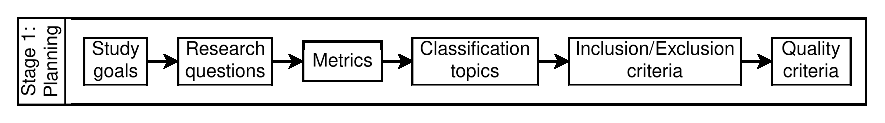
\includegraphics[scale=1.0]{resources/figures/sms-Etapa-1.eps}
	\caption{Components of the planning stage}
	\label{fig:PlanningStageOverview}
\end{figure}

% 4.1.1
%sub-subsection - study objectives
\subsubsection{Study Objectives}
Considering the aspects described in the motivation section, two objectives were defined for the study and are detailed in Table~\ref{table:Goals}.

%Table 1 
\begin{table}
	\tbl{Goals of the SMS.}
	{\begin{tabular}{p{1cm}p{6.8cm}} \toprule
			\textbf{Goal} & \textbf{Description}                                                                                                                                                                                                                                                                                                                                 \\
			\midrule
			\textbf{G1}   & Classify works related to HTCondor universes according to their application and impact in common IT domains, such as distributed and parallel computing, HTC, software development, virtualization and microservices, computer networks, computational infrastructure, artificial intelligence, data analysis, computational thinking, among others. \\
			\textbf{G2}   & Identify and categorize works related to HTCondor universes as a tool to enhance academic functions (AF) such as research, teaching, and industry collaboration.                                                                                                                                                                                     \\
			\bottomrule
		\end{tabular}}
	\label{table:Goals}
\end{table}


% 4.1.2
%sub-subsection - research question
\subsubsection{Research Question}
For the construction of the research questions (RQs), the GQM and PICOC models~\cite{Needleman20026, Petticrew2008systematic} were used. This model allows us to establish the aspects ``Population,'' ``Intervention,'' ``Comparison,'' ``Outcomes,'' and ``Context''. This ensures situating the study in an appropriate environment and delivering value. See Table \ref{table:PICOC}.

Drawing on the PICOC model, two research questions (RQs) were formulated, as presented in Table~\ref{table:RQs}.

% Table 2 
\begin{table}
	\tbl{Application of the PICOC model}
	{\begin{tabular}{p{2.0cm}p{8.0cm}} \toprule
			\textbf{Component}    & \textbf{Description}                                                                                                                                         \\
			\midrule
			\textbf{Population}   & Works related to HTCondor universes that leverage academic functions and impact common IT domains.                                                           \\
			\textbf{Intervention} & To identify and classify a set of Works related to HTCondor universes that leverage academic functions and impact common IT domains                          \\
			\textbf{Comparison}   & Documented project cases; Compliance with inclusion and exclusion criteria; Appearance in selected databases.                                                \\
			\textbf{Outcomes}     & Taxonomy that organizes works related to HTCondor universes that enhance academic functions, according to their application and impact in common IT domains. \\
			\textbf{Context}      & HTCondor universes that enhance academic functions, according to their application and impact in common IT domains.                                          \\
			\bottomrule
		\end{tabular}}
	\label{table:PICOC}
\end{table}

% Table 3
\begin{table}
	\tbl{Research questions of the SMS.}
	{\begin{tabular}{p{0.5cm}p{1.4cm}p{6.0cm}p{4.5cm}} \toprule
			\textbf{Goal} & \textbf{Research Question} & \textbf{Description}                                                                                                                                                                                                                                                                                                & \textbf{Motivation}                                                                                                                                                  \\
			\midrule
			G1            & RQ1                        & What works related to HTCondor universes have an impact on common IT domains such as distributed and parallel computing, HTC, software development, virtualization and microservices, computer networks, computational infrastructure, artificial intelligence, data analysis, computational thinking, among others?. & To recognize how HTCondor universes that have an impact on common IT domains are structured, identify their applications, and determine their contextual motivation. \\
			G2            & RQ2                        & How do HTCondor universes specifically support teaching, research assessment, and industry collaboration workflows?.                                                                                                                                                                                         & To recognize how HTCondor universes that enhance academic functions are structured, identify their applications, and determine their contextual motivation.          \\
			\bottomrule
		\end{tabular}}
	\label{table:RQs}
\end{table}

% 4.1.3
%sub-subsection - metrics
\subsubsection{Metrics}
The SMS metrics were defined using a quantitative approach in accordance with our classification structure. The details of the metrics are shown in Table \ref{table:Metrics}. The criteria established restrict documents to a validity period of 28 years because of the scarcity of documentation on HTCondor and to provide readers with a broad range of articles, from foundational works to more recent studies. In addition, the study type was limited to primary studies indexed in recognized databases to ensure peer-review rigor.

% Table 4
\begin{table}
	\tbl{Metrics of the SMS}
	{\begin{tabular}{p{1cm}p{6.8cm}} \toprule
			\textbf{Metric} & \textbf{Description}                                                                            \\
			\midrule
			\textbf{M1}     & Number of works selected in the final stage of the SMS.                                         \\
			\textbf{M2}     & Popularity of each Universe in the works selected in the final stage.                           \\
			\textbf{M3}     & Percentage of works selected in the final stage with respect to the number of works considered. \\
			\textbf{M4}     & Percentage of works selected in the final stage, contributed by each database.                  \\
			\bottomrule
		\end{tabular}}
	\label{table:Metrics}
\end{table}

% 4.1.4
%sub-subsection - research topics
\subsubsection{Topics}
The RQs and the PICOC model serve as the baseline for selecting the classification topics used in this study. The topics are as follows: Artificial Intelligence (AI), Cloud Computing, Containerization, Grid Computing, High Performance Computing (HPC), Java, Virtualization, Kubernetes, Networks, Parallelism, Docker, High Throughput Computing (HTC), Teaching, Research, and Industry.

% 4.1.5
%sub-subsection - inclusion and exclusion criteria
\subsubsection{Inclusion and Exclusion Criteria}
The inclusion and exclusion criteria defined for the study are shown in Table \ref{table:Criteria}.

% Table 5
\begin{table}
	\tbl{Inclusion and exclusion criteria for database search}
	{\begin{tabular}{p{2.7cm}p{5cm}p{5cm}} \toprule
			\textbf{Category}   & \textbf{Inclusion Criteria}                                                                                                                        & \textbf{Exclusion Criteria}                                                                                                        \\
			\midrule
			Fields              & All.                                                                                                                                               & -                                                                                                                                  \\
			Type of publication & Research articles.                                                                                                                                 & Theses, book chapters, books, journals, \textit{proceedings}, \textit{papers}, and anything not covered by the inclusion criteria. \\
			Area or discipline  & Computer science, Engineering (in the ACM database it is assumed that all articles are related to these subjects since filtering is not possible). & Areas unrelated to computer science and engineering.                                                                               \\
			Period              & From 1996 to 2024.                                                                                                                                 & -                                                                                                                                  \\
			Language            & English.                                                                                                                                           & -                                                                                                                                  \\
			\bottomrule
		\end{tabular}}
	\label{table:Criteria}
\end{table}

The temporal scope of this systematic mapping study spans from 1996 to 2024, a period determined empirically through the comprehensive search process rather than predetermined theoretical considerations. Initially, the search strategy employed a broader temporal framework extending back to 1980 to ensure comprehensive coverage of all potentially relevant literature in the domain of distributed computing and high-throughput computing systems. However, the systematic application of our search protocols across the selected databases revealed that the earliest study meeting our inclusion criteria and addressing HTCondor universes was published in 1996. This finding aligns with the historical development trajectory of HTCondor, which evolved from the original Condor project initiated at the University of Wisconsin-Madison in the late 1980s, with the first substantial academic publications emerging in the mid-1990s as the system matured and gained adoption in the scientific computing community. Consequently, the 28-year period from 1996 to 2024 represents the complete temporal landscape of scholarly literature specifically addressing HTCondor universe implementations, providing a comprehensive foundation for understanding the evolution, application, and impact of these execution environments across diverse computational domains. This data-driven approach to temporal boundary setting ensures that our analysis captures the full breadth of available evidence while maintaining methodological rigour in the systematic mapping process.


%4.1.6 Quality Criteria

\subsubsection{Quality Criteria}
At the end of the planning stage, we have adopted three quality criteria.

% ###### CVI ######## 
The first quality criterion is an adaptation of the CVI (Content Value Index)~\cite{Almanasreh2019214, yaghmaei2003content}. In this case, we judged the documents by identifying those most relevant to the SMS.~We used a quantitative scale from 0 to 5 for this index, where 0 implies a low relationship of the studies with the SMS goals and 5 implies a high relationship. See formula (\ref{equation:CVI}). $k$ is the odd total workers, $f(n)$ is the value assigned by the worker $n$.

\begin{equation}
	\label{equation:CVI}
	CVI = \frac{\sum_{n=1}^{k} f(n)}{k}
\end{equation}

%###### SCI ######
The second quality criterion considers the number of citations of each study relative to its publication age (A)., which we call SCI (Study Citation Index). See  formula (\ref{equation:SCI}). $C$ is Citations between 1996 to 2024, and $A$ is \textit{Age of study}. With this formula, we seek to balance the citation of the studies. Thus, a citation in a  paper from 2024 has a higher value than in a paper from 1996.


\begin{equation}
	\label{equation:SCI}
	SCI = \frac{C}{A}
\end{equation}


\hbox{}
The third quality criterion used corresponds to the relationship of the studies with the research questions; this criterion is named IRRQ (\textit{Index of Relationship to Research Questions}), see formula (\ref{equation:IRRQ}), where \textit{N} corresponds to the number of RQs to which the study is related. Subsequently, \textit{N} is divided by 2, as this is the number of research questions defined.

\begin{equation}
	\label{equation:IRRQ}
	IRRQ = \frac{N}{2}
\end{equation}

